\section*{Creating Files (\texttt{open} system call)}
\begin{lstlisting}[language=c]
// new: `open' also create a file if it doesn't exist yet
int fd = open("foo", O_CREAT|O_WRONLY|O_TRUNC, S_IRUSR|S_IWUSR);
// old: equivalent to calling open() with O_CREAT | OWRONLY | O_TRUNC
int fd = creat("foo"); // option: add second flag to set permissions
\end{lstlisting}
Flags and parameters:
\begin{enumerate*}[label={\alph*.},font={\color{red!50!black}\bfseries}]
\item \texttt{O\_CREAT} creates the file if it doesn't exit
\item \texttt{O\_WRONLY} ensures it can only be written to and
\item if the file already exits, truncate it to a size of zero bytes $\to$ removing any existing content (\texttt{O\_TRUNC})
\end{enumerate*}
The 3rd parameter specifies permissions, making the file readable and writable by the owner. On success, return a \mb{file descriptor}\\
\begin{minipage}{.45\linewidth}
\begin{lstlisting}[language=c]
struct proc {
  // other fields ...
  // array of open file
  struct file *ofile[NOFILE];
  // other fields ...
} // Linux uses task_struct
\end{lstlisting}
\end{minipage}
\begin{minipage}{.55\linewidth}
  \flushleft
  \begin{itemize}
  \item xv6 keeps an \texttt{array[NOFILE] of files}, indexed by file descriptor
  \item tracks which files are opened on a per-process basis
  \item each entry a ptr to a \texttt{struct file} to track the file being read/written
  \end{itemize}
\end{minipage}
\section*{Reading \texttt{read()} and Writing \texttt{write()} files (sequentially: start $\to$ end)}
\begin{lstlisting}[language=bash]
# run strace cat foo in terminal; get below output (relevant only)
# O_LARGEFILE -> 64-bit offset; 3 -> returned file descriptor
open(``foo'', O_RDONLY|O_LARGEFILE) = 3
# read fd 3 into buffer ``hello\n'' of size 4KB; returned bytes read: 6
read(3, ``hello\n'', 4096)              = 6
# `cat' may call `write' or `printf' which `write' to stdout (1)
write(1, ``hello\n'', 6)                = 6 # write to stdout
hello
read(3, ``'', 4096)                     = 0 # nothing to read, returns 0
close(3)                                = 0 # indicate done
\end{lstlisting}
Writing a file in similar steps:
\begin{enumerate*}[label={\alph*.},font={\color{red!50!black}\bfseries}]
\item a file is opened for writing,
\item then call \texttt{write()} syscall, perhaps repeatedly for larger files,
\item then \texttt{close()}
\end{enumerate*}
\section*{Reading/Writing not sequentially (current offset updated in 2 ways)}
\begin{lstlisting}[language=c]
// look up specific word -> read from random offsets within a file
off_t lseek(int fildes, off_t offset, int whence);
// If whence is SEEK_SET, the offset is set to offset bytes.
// If whence is SEEK_CUR, offset = its current location + offset bytes
// If whence is SEEK_END, offset = file size + offset bytes
\end{lstlisting}
\begin{enumerate}
\item \emph{explicitly} with \texttt{lseek}, which changes the offset as specified above
\item when R/W of $N$ bytes, \texttt{curr\_offset += N}: \emph{implicitly} updates offset
\end{enumerate}
\begin{minipage}{.3\linewidth}
\begin{lstlisting}[language=c]
struct file {
  int ref; // sharing
  char readable;
  char writable;
  struct inode *ip;
  uint off;
}; // simplified def
\end{lstlisting}
\end{minipage}
\begin{minipage}{.7\linewidth}
  \flushleft
  \begin{itemize}
  \item OS uses this to determine whether opened file is readable or writable or both
  \item \texttt{struct inode ip} points to the underlying file
  \item These file structs represent all of the currently opened files in the system; together, they are sometimes referred to as the \mb{open file table}
  \end{itemize}
\end{minipage}
\begin{minipage}{.45\linewidth}
\begin{lstlisting}[language=c]
struct {
  struct spinlock lock;
  struct file file[NFILE];
} ftable;
\end{lstlisting}
\end{minipage}
\begin{minipage}{.55\linewidth}
  \flushleft
  \begin{itemize}
  \item open file table keeps \texttt{struct file}
  \item in most cases, there's 1-to-1 mapping from \texttt{fd} to an entry in OFT, but it may be shared
  \end{itemize}
\end{minipage}
\begin{itemize}
\item mutil procs read same file at same timw: each has its own OFT entry
\item each logical R/W of a file is independent, with its own current offset
\end{itemize}
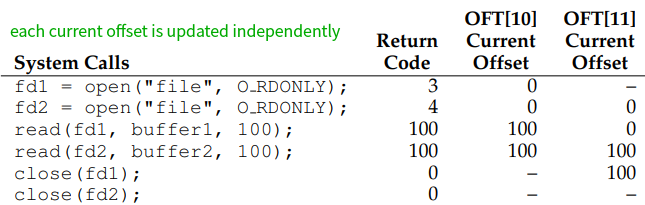
\includegraphics[width=\linewidth]{imgs/fs_read_conc}
\section*{Shared File Table Entries \texttt{fork} and \texttt{dup}}
\begin{minipage}{.4\linewidth}
  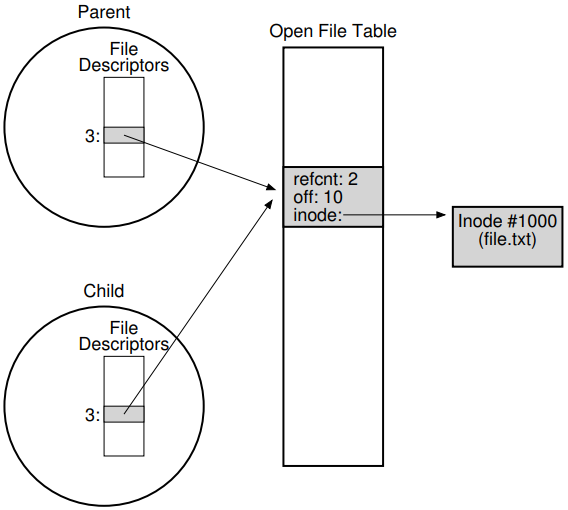
\includegraphics[width=\linewidth]{imgs/fs_shared_ote}
\end{minipage}
\begin{minipage}{.6\linewidth}
  \flushleft
  \begin{itemize}
  \item when parent process \texttt{fork()} a child, child shares its parent's OTF
  \item each process has its own independent copy of file descriptor
  \item \texttt{ref} in \texttt{struct file} keeps \# descriptors sharing the entry; only when both processes close file (or exit) will the entry be removed
  \item \texttt{dup()} creates new fd that refers to same OFT entry (file) as an existing fd
  \end{itemize}
\end{minipage}
\section*{Writing Immediately \texttt{fsync()}}
\begin{itemize}
\item  For performance reasons, the file system may \textbf{buffer} \texttt{write()} to memory for a short while before actually writing it to disks
\item  Drawback: some writes may be lost if the system crashes (power loss); DBSM recovery protocol may require ability to force write to disk
\item syscall \texttt{fsync()} tells file system to force writing all \textbf{dirty} data to disk
\item May need to \texttt{fsync()} both a file and the directory containing it
\end{itemize}
\begin{itemize}
\item Another method to R/W a file: map it to memory using syscall \texttt{mmap()}
\item R/W to a file becomes load/store to its memory-mapped locations
\item \texttt{msync()} to flush changes in memory to the file system
\item Key benefits:
\begin{enumerate*}[label={\alph*.},font={\color{red!50!black}\bfseries}]
\item creates a direct link btwn file byte offsets (backing file) and virtual addr in calling process
\item combines file persistence and memory-like access semantics;
\item enables persistent memory programming;
\item Makes apps faster by avoiding RAM-disk data changes
\end{enumerate*}
\end{itemize}
\section*{Renaming Files: \texttt{rename()} (atomic operation during sys crashes)}
\begin{itemize}
\item on command line: \texttt{mv}; use syscall \texttt{rename(char *old, char *new)}
\item file will have either old or new name; \emph{no} partial states possible
\item common file update process:
  \begin{enumerate*}[label={\alph*.},font={\color{red!50!black}\bfseries}]
  \item write new content to tmp file;
  \item sync temp file to disk;
  \item rename tmp file to target (used by text editors)
  \end{enumerate*}
\begin{lstlisting}[language=c]
int fd = open("foo.txt.tmp", O_WRONLY|O_CREAT|O_TRUNC,
              S_IRUSR|S_IWUSR);
write(fd, buffer, size); // write out new version of file
fsync(fd); close(fd); rename("foo.txt.tmp", "foo.txt");
\end{lstlisting}

\item key benefits:
  \begin{enumerate*}[label={\alph*.},font={\color{red!50!black}\bfseries}]
  \item ensures atomic updates
  \item prevents data loss
  \item old file remains until update complete (for safe file modifications)
  \end{enumerate*}
\end{itemize}
\section*{Getting Info About Files \texttt{stat()} and Remove (\texttt{unlink()} syscall)}
\begin{minipage}{.7\linewidth}
\begin{lstlisting}[language=c]
struct stat {
  dev_t st_dev; // ID of device containing file
  ino_t st_ino; // inode number
  mode_t st_mode; // protection
  nlink_t st_nlink; // number of hard links
  uid_t st_uid; // user ID of owner
  gid_t st_gid; // group ID of owner
  dev_t st_rdev; // device ID (if special file)
  off_t st_size; // total size, in bytes
  blksize_t st_blksize; // blksize for filesys I/O
  blkcnt_t st_blocks; // number of blks allocated
  time_t st_atime; // time of last access
  time_t st_mtime; // time of last modification
  time_t st_ctime; // time of last status change
};
\end{lstlisting}
\end{minipage}
\begin{minipage}{.3\linewidth}
  \flushleft
  \begin{itemize}
  \item metadata keeps info on each file in sys
  \item accessed via \texttt{stat()} and \texttt{fstat()}
  \item takes pathname and fd as input
  \item inode struct:
    \begin{enumerate*}[label={\alph*.},font={\color{red!50!black}\bfseries}]
    \item stored persistently on disk
    \item active inodes cached in RAM to speed up access
    \item acts as fs's data struct
    \end{enumerate*}
  \end{itemize}
\end{minipage}
\section*{Directory Syscalls for Making, Reading, Deleting Directories}
\begin{itemize}
\item dirs format is fs metadata $\to$ user can’t modify its bytes arbitrarily
\item updates \emph{only} through \mr{indirect} actions:
  \begin{enumerate*}[label={\alph*.},font={\color{red!50!black}\bfseries}]
  \item \texttt{mkdir}
  \item \texttt{opendir}
  \item \texttt{rmdir}
  \item \texttt{readdir} to read dir entries (files, subdirs)
  \item \texttt{closedir}
  \end{enumerate*}
\item \texttt{rmdir()} requires the dir to be empty: only has \texttt{.} and \texttt{..} before deleting it $\to$ removing non-empty causes \texttt{rmdir()} to fail
\item dirs are light on info: just mapping name to inode number, plus a few other details $\to$\ texttt{ls -l} calls \texttt{stat()} on each file to get more info
\end{itemize}
\begin{lstlisting}[language=c]
struct dirent {
  char d_name[256];           // filename
  ino_t d_ino;                // inode number
  off_t d_off;                // offset to the next dirent
  unsigned short d_reclen; // length of this record
  unsigned char d_type;       // type of file
};
\end{lstlisting}
\section*{Hard, Soft links with \texttt{link()} and \texttt{unlink()}}
\begin{itemize}
\item \texttt{ln} uses \texttt{link()} syscall that takes two args: old and new pathnames
\item \mo{link} creates a new file name to refer to the old, existing one (not copied in any way, just two human-readable names referring to the same file)
\item creating a file is doing two things:
  \begin{enumerate*}[label={\alph*.},font={\color{red!50!black}\bfseries}]
  \item make inode struct that tracks all relevant info about the file (size, blk location on disk, etc)
  \item \emph{link} a human-readable name to that file and put that link into a directory
  \end{enumerate*}
\item file system see no difference between original and new files
\item Each inode keeps a \mb{reference count} (link count) to track how many file names associated with it
\item \texttt{unlink()} removes ``link'' btwn human-readable name and inode number, decrements ref count $\to$ iif \texttt{ref\_cnt == 0}, fs truly deletes the file
\item \textbf{can't} hard link to a directory (for fear of cycle in directory tree)
\item \textbf{can't} hard link to files on other disk partitions $\because$ inode numbers only unique within a particular file system, not across file systems
\end{itemize}
\begin{lstlisting}[language=bash]
prompt> echo hello > file           # create a file with some content
prompt> stat file                   # use `stat' to see the reference count
... Inode: 67158084 Links: 1 ...
prompt> ln file file2               # hard link to an existing file
prompt> stat file
... Inode: 67158084 Links: 2 ...  # reference count incremented by 1
\end{lstlisting}
\begin{itemize}
\item symbolic (soft) link is a file itself of a different type (not \texttt{-} or \texttt{d}, but \texttt{l})
\item soft links \emph{only} refers to filename, \texttt{file\_size == bytes of filename}
\item shorter pathname $\to$ small soft link file, longer pathname $\to$ larger file
\item \mr{dangling reference}: removing original file causes soft link to points to pathname that no longer exists
\end{itemize}
\section*{Access Control encoded in Permission Bits}
\begin{itemize}
\item \textbf{3} groups of 3-bit data, controlling \textbf{r}ead/\textbf{w}rite/e\textbf{x}ecute access
\begin{lstlisting}[language=bash]
prompt> ls -l foo.txt
-rw-r--r-- 1 remzi wheel 0 Aug 24 16:29 foo.txt
# -: regular file; d: directory; l: symbolic link
\end{lstlisting}
\item one more extra group of 3-bit for setuid/setgid bits
\begin{lstlisting}[language=bash]
# setuid (0o4000): file owner; setgid (0o2000); sticky bit (0o1000)
chmod 4755 myfile  # Sets setuid and rwxr-xr-x
\end{lstlisting}
\item for directories, its execute bit enables a user (or group/others) to \texttt{cd} into the given directory and if with writable bit, create files therein
\end{itemize}
\begin{minipage}{.5\linewidth}
  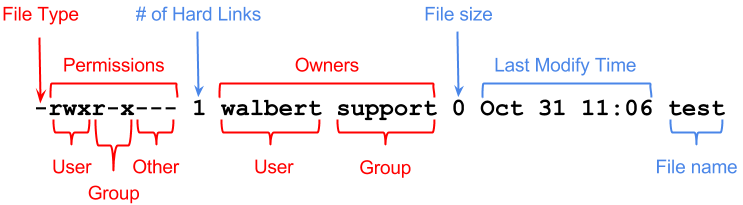
\includegraphics[width=\linewidth]{imgs/file_perm2}
\end{minipage}
\begin{minipage}{.5\linewidth}
  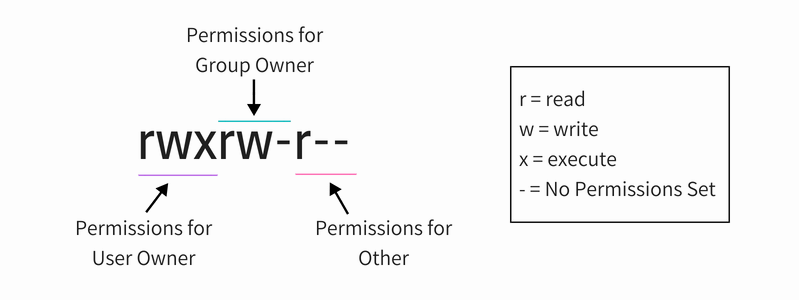
\includegraphics[width=\linewidth]{imgs/file_perm1}
\end{minipage}
\section*{Making and Mounting A File System}
\begin{itemize}
\item \texttt{mkfs} accepts a device (e.g. \texttt{/dev/sda1}) and a fs type (e.g. \texttt{ext4}) $\to$ creates an empty fs starting with root dir onto that disk partition
\item \texttt{mount} (uses syscall \texttt{mount()}) takes an existing directory as a target \textbf{mount point} and essentially pastes a new fs onto the directory tree at that point, making new fs accessible within the uniform fs tree $\to$ unifies all file systems into one tree $\to$ uniform and convenient naming
\item run \texttt{mount} to see what is mounted and at which points on your sys
\end{itemize}
